\documentclass[a4paper,11pt,oneside]{book}

\usepackage[english]{babel}
\usepackage[showframe=false]{geometry}
\usepackage[usenames,dvipsnames]{xcolor}
\usepackage[utf8]{inputenc}
\usepackage[T1]{fontenc}
\usepackage{changepage}
\usepackage[]{algorithm2e}
\usepackage{amssymb}
\usepackage{amsmath}
\usepackage{graphicx}
\usepackage{listings}
\usepackage{verbatimbox}
\usepackage{ulem}
\usepackage{fancyvrb}
\usepackage{float}
\usepackage{hyperref}
\usepackage[parfill]{parskip}
\usepackage{tikz}
\usepackage{pdflscape}
\usepackage{minted}
\usepackage{titlesec}
\usepackage{titleps}
\usepackage{lastpage}
\usepackage{fancyhdr}
\usepackage{etoolbox}
\usepackage[]{algorithm2e}
%Following overwrites the page style for chapters
\patchcmd{\chapter}{\thispagestyle{plain}}{\thispagestyle{ruledChapter}}{}{}

%New page style for chapters
\newpagestyle{ruledChapter}{
	\setfoot{}{\thepage\ of \pageref{LastPage}}{}
	\footrule
	\renewcommand\makefootrule{\color{black}\rule[\baselineskip]{\linewidth}{0.4pt}}
}
%New page style for rest
\newpagestyle{ruled}{
	\sethead{\raggedright \chaptername\ \thechapter :\ \chaptertitle}{}{}
	\headrule
	\setfoot{}{\thepage\ of \pageref{LastPage}}{}
	\footrule
	\renewcommand\makeheadrule{\color{black}\rule[-.3\baselineskip]{\linewidth}{0.4pt}}
	\renewcommand\makefootrule{\color{black}\rule[\baselineskip]{\linewidth}{0.4pt}}
}

\expandafter\def\csname PY@tok@err\endcsname{}
\newcommand{\HRule}{\rule{\linewidth}{0.5mm}}
\newcommand{\specialcell}[2][c]{%
  \begin{tabular}[#1]{@{}c@{}}#2\end{tabular}}

\addtocontents{toc}{\protect\thispagestyle{empty}}

\title{}
\author{}
\date{} 

\begin{document}
\begin{titlepage}
\begin{center}

%-----------------------------------------------------------------
%							FRONTPAGE
%-----------------------------------------------------------------
\thispagestyle{empty}

\includegraphics[width=0.55\textwidth]{logo.pdf}\\[1cm]    
\textsc{\Large DM818 Assignment 2}\\[0.5cm]

% Title
\begin{Huge}
\textbf{Parallel Particle Simulation}
\end{Huge}

\vspace{4cm}

% Author and supervisor
\begin{minipage}{1\textwidth}
\begin{center}
\emph{}\\

Dan \textsc{Sebastian Thrane}\\
\verb!<dathr12@student.sdu.dk>!\\

Lars \textsc{Thomasen}\\
\verb!<latho12@student.sdu.dk>!\\

\end{center}
\end{minipage}
\begin{minipage}{0.4\textwidth}
\end{minipage}

\vfill

% Bottom of the page
{\large Winter 2015}\\

\end{center}
\end{titlepage}

%-----------------------------------------------------------------
%							   TOC
%-----------------------------------------------------------------
\renewcommand{\contentsname}{Table of Contents}
\tableofcontents
\thispagestyle{empty}

%-----------------------------------------------------------------
%						  ACTUAL REPORT
%-----------------------------------------------------------------
\pagestyle{ruled}
\chapter{Introduction}
\setcounter{section}{1}

This reports documents the second mandatory assignment for the course DM818 Parallel Computing. In this assignment we
were given a particle simulation which runs in $O(n^{2})$ time, and were asked to code the following:

\begin{enumerate}
\item Change the implementation such that it runs in $O(n)$ time.
\item Parallelize the changed code using either OpenMP, PThreads, or MPI.
\end{enumerate}

In order to measure proper performance gain, we need to optimize the serial algorithm first, and then parallelize it
such that the comparison stays fair. It would be easy to show a massive performance gain if the algorithm for the
parallel implementation is vastly superior to the one used for linear.
 
\section{Work Load}

% A statement of who contributed with what.

The distribution of the workload has been equal, and pair programming in the IMADA terminal room have been the preferred
method throughout this project.

\chapter{A Linear Algorithm}

% A plot in log-log scale that shows that your serial and parallel codes run in O(n) time and a description of the data
% structures that you used to achieve it.

\section{The Base Algorithm}

The given algorithm for the serial implementation (and the parallel versions) are as follows, clearly running in
$O(n^{2})$ runtime. This was unacceptable and thus a new algorithm has been developed.

\begin{minted}[frame=single,linenos=true]{c}
for(int i = 0; i < n; i++) {
  particles[i].ax = particles[i].ay = 0;
  for (int j = 0; j < n; j++) {
    apply_force(particles[i], particles[j]);
  }
}
\end{minted}

The problem with this algorithm is that it applies forces between all pairs of particles, while the rules for the
particle simulation states that any particle may only be affected by nearby particles.

\section{The new algorithm}

The range for interaction for the particles was reduced to a smaller value, denoted as the ``cutoff'' value. This cutoff
value was showcased as a grey border on a particle in the assignment.

\begin{figure}[H]
  \centering
  \begin{minipage}[b]{0.4\textwidth}
    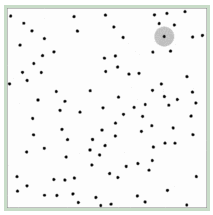
\includegraphics[width=\textwidth]{cutoff.png}
    \caption{Snapshot of the GIF from the assignment showcasing the influence ring.}
  \end{minipage}
\end{figure}

Having a reduced area of interaction, allows us to reduce the amount of particles influencing the amount of force needed
to be applied to a given particle, thus we can reduce the inner for-loop greatly.

In order to reduce the loop it is necessary to know which particles are within (or at least close by) the particle we
want to apply the force. To do this we needed to develop a data structure, to keep track of where the particles are
positioned.

In order to track the location of the particles, the coordinate system is divided into a grid of cells. Each cell holds
some number of particles within a sub-grid of the entire universe. The sizes of the cells are chosen to match the
``cutoff'' value, such that we only need to check the neighboring cells for collisions with a particle.

\begin{figure}[H]
  \centering
  \begin{minipage}[b]{0.4\textwidth}
    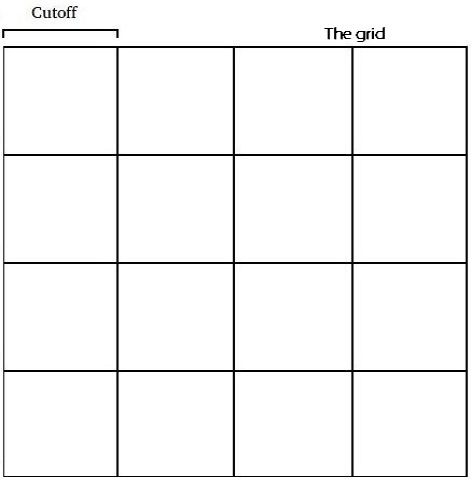
\includegraphics[width=\textwidth]{grid.jpg}
    \caption{The grid structure, showcasing the size of a single position equals the cutoff size.}
  \end{minipage}
  \begin{minipage}[b]{0.4\textwidth}
    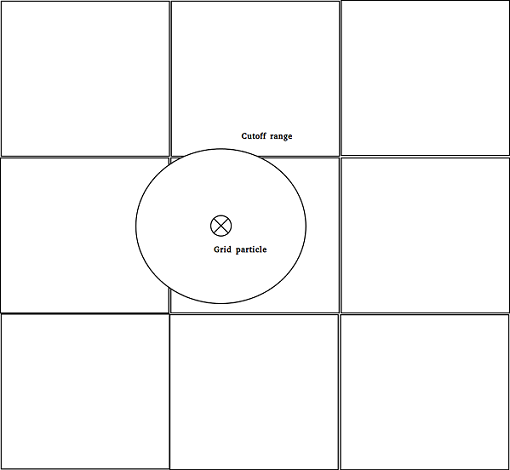
\includegraphics[width=\textwidth]{gridexample.png}
    \caption{A particle located inside a grid positions, and its influence range.}
  \end{minipage}
\end{figure}

Initially all particles are added to the grid. When updates are performed on a particle, it will be moved  to the
appropriate cell as well.

\section{Implementing the Grid Approach}

% TODO Not sure about this section

The implementation uses a separate file named \verb!grid.cpp! and \verb!grid.h!. These files holds the data structure
and a series of helper methods that allows us to add, get and remove particles to the grid. The grid itself is 2D array
of particles.

Whenever we move a particle, we simply remove the particle from the grid completely, and then add it back in. This way
the old position is removed, and the new position is calculated from the particles new position when added again. 

\section{Performance of the New Algorithm}

Below is a graph plotted for different times (see appendix A) showcasing how the $O(n^{2})$ and $O(n)$ algorithms do
versus each other. It is easy to see that the $O(n)$ is indeed linear. Note that bigger sizes did not terminate in
reasonable time for the $O(n^{2})$ algorithm.

\begin{figure}[H]
  \centering
  \begin{minipage}[b]{0.9\textwidth}
    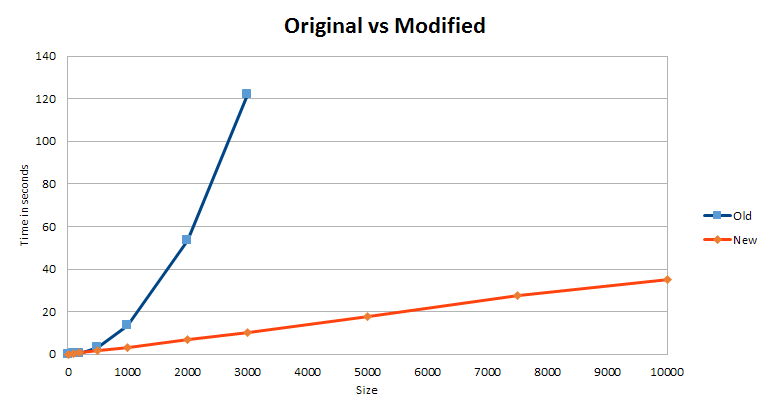
\includegraphics[width=\textwidth]{graph_regular.png}
    \caption{The original $O(n^{2})$ algorithm (blue) versus the new $O(n)$ algorithm (red).}
  \end{minipage}
\end{figure}

\chapter{Parallelization using MPI}

Throughout this chapter we will discuss how our serial implementation was parallelized. The parallelization was done
using MPI, and we will be referring to concept found in this library whenever relevant.

\section{Model for Communication}

We would like to share the work onto multiple processors, to parallelize our serial implementation. Looking at our
implementation it seems obvious to give each processor a set of cells to be responsible for, instead of giving each
processor a set of particles to be responsible for. By letting each processor be responsible for a zone, it can
perform most of the work completely locally, since each cell can only contain particles that will be affected by
particles in neighboring zones. This means that only particles lying in a cell at the border of the zone, may be
affected by a cell not owned by the local processor.

There are several ways in which the grid may be divided into zones for the processors. For the sake of simplicity
each processor is given some number of rows in the grid, for which they are responsible. This means that any processor
will have at most two neighboring processors, the one responsible for the rows above, and the one for the rows below.

\begin{figure}[H]
  \centering
  \begin{minipage}[b]{0.9\textwidth}
    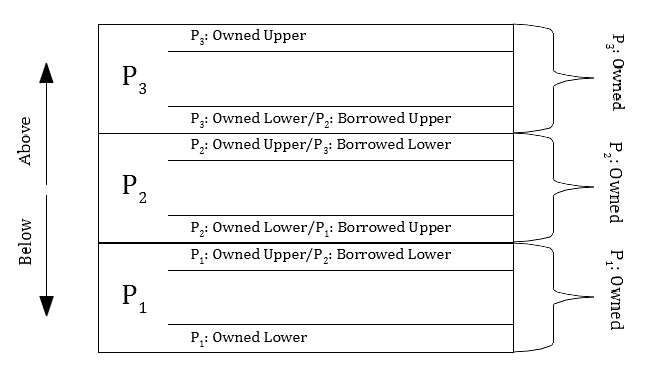
\includegraphics[width=\textwidth]{zones.png}
    \caption{Splitting the grid into zones.}
  \end{minipage}
  \label{fig:zones}
\end{figure}

% TODO Wording

To deal with the problems of the zones lying at the border of a zone, we've introduced the concept of borrowed and owned
zones as shown in figure \ref{fig:zones}. These zones are exactly correspond to exactly one row in the grid. Each
processor will contain up-to-date ``borrowed'' copies of these zones. The figure how each processor identifies the
different zones. Each processor will have to communicate with its neighbors to keep these zones in sync.

\section{Initializing the System}

The initial system is initialized at the root. Once all the particles have been created, a local grid is created, like
in the serial version. This gives us the initial distribution, which is then distributed to all the processors in the
system using \verb!MPI_Scatterv!.

\section{Synchronization of Nodes}

As discussed previously, each processor will need to keep synchronized copies of zones that they borrow
from each other. Since we in every iteration may make a change to these zones, we will need to perform this
synchronization step in every single iteration as well. The synchronization process is two-fold, first we gather up-to-
date information, and then we merge our information to get a correct picture of the system.

\textbf{Step 1: Synchronize Processors}

At the beginning of every iteration, we will need to synchronize all processors, such that they are all ready for the
next iteration. Once they are ready for the next iteration, we may begin exchanging information. This synchronization
can be done using the \verb!MPI_Barrier! procedure.

\textbf{Step 2: Prepare for Exchange with Neighbors}

A processors' neighboring processes will expect a complete image of how the zone it is borrowing looks. This message 
needs to be prepared, such that we can transmit it, this process consists solely of packing all the particle into a 
single buffer.

Before beginning the exchange, we will also clear out any particles that reside inside of the borrowed zones. This is
done since we will receive a completely new zone from our neighbors.

\textbf{Step 3: Exchange Message with Neighbors}

Once the messages are ready, we may exchange data with our neighbors. For efficiency reasons we use \verb!MPI_SendRecv!,
which allows for simultaneously sending and receiving data between two nodes. MPI requires that both parties involved in
the transfer, call this function with each other as arguments. For this reason, the following pattern has been
established: processors with an even rank communicate with the processor above it first, while processors with an odd
rank will communicate with the processor below first. The exchange process between two processors go like this:

\begin{enumerate}
	\item Exchange sizes (in particles) of zones
	\item Exchange the particles, this exchange requires the knowledge of how many particles we will receive
	\item Exchange sizes of local insertions into borrowed zones
	\item Exchange particles involved in local insertions into borrowed zones
\end{enumerate}

It should also be noted that this means that the synchronization process for the system as a whole, will only take the
time of communicating with each neighbor, since these are all done in parallel.

\textbf{Step 4: Update the World}

We have already discussed that we share our owned zones with our neighbors. The reason for this fairly simple, we're the
ones responsible for updating these zones, hence we are the ones capable of telling our neighbors about updates made in
it.

However, it is also possible for particles to migrate from one processor to another. Hence we need to track whenever we
perform an insertions of particles from our owned zone into a borrowed zone. These particles are all tracked in a
separate buffer, and exchanged with the neighbor in step 3.

The insertions that we receive from our neighbors are then merged together with our own local view to give a completely
up-to-date view of the system.

\textbf{Step 5: Cleanup}

Finally we clear out our local insertions from an owned zone into a borrowed zone. Such that we're ready for the next 
iteration.

\section{Running the Simulation and Combining the Result}

The simulation step itself is left mostly unchanged from the original serial implementation. It should however be noted
that we only have to directly look at the particles we own ourselves. That is we do not need to loop directly over the
particles in the borrowed zones, since if any of our owned particles collide with them, then this will be picked up when
we look at the neighboring cells.

While the simulation is running, we write down where are particles are. To be able to merge the particles later, we have
had to add an ID number to every particle, such that we may track any particle, even if it goes through several
processors. Once the simulation is done, it is collected at the root node using \verb!MPI_Gatherv!, sorted per
iteration, and ID, and saved to the output file.

\section{Limitations}

The technique used for distributing the cells to each processor, puts some limitations to the number of processors one
can effectively use with the system. The current implementation allows for at most as many processors as there are rows.
And when hitting this case, we won't be very effective, since we will hold twice as many borrowed cells, that we hold
owned cells. The system could allow for more processors by letting the zones be smaller squares, that do not need to
have the same width as the entire grid. This does however come at the cost of having up to four neighbors instead of at
most two and the increase complexity in communicating.

\section{Performance}
This section is used to document two aspects:

\begin{enumerate}
  \item Overall performance 
  \item Breakdown of time used in a single run
\end{enumerate}

Like previously, in order to confirm that the implementation is still linear, we can plot the time against the input size
and visually see the result.

\begin{figure}[H]
  \centering
  \begin{minipage}[b]{0.9\textwidth}
    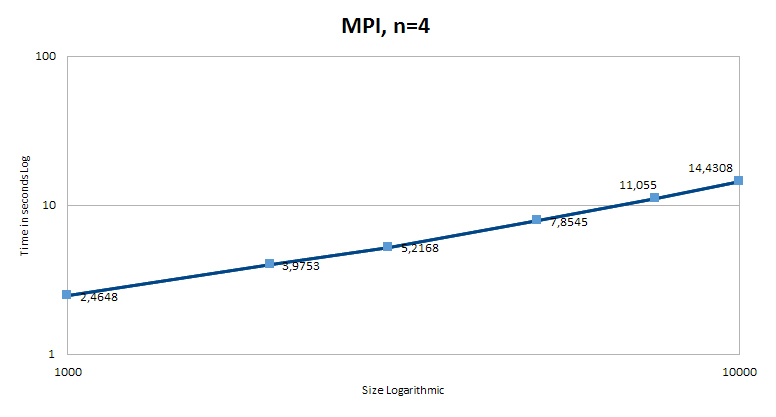
\includegraphics[width=\textwidth]{mpi_log.png}
    \caption{Runtimes for the MPI implementation using 4 processes.}
  \end{minipage}
\end{figure}

\begin{figure}[H]
  \centering
  \begin{minipage}[b]{0.9\textwidth}
    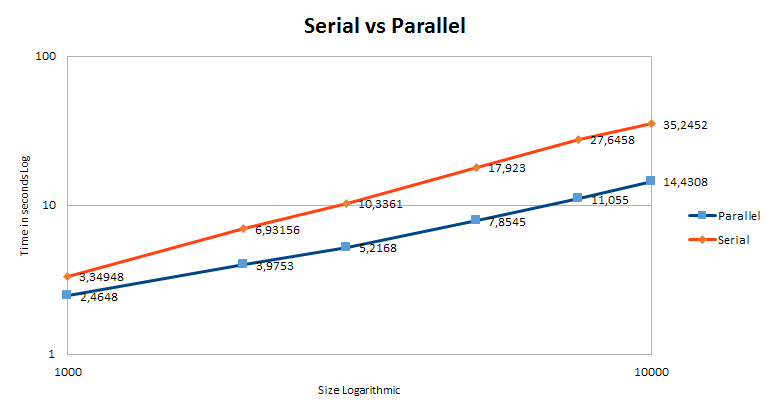
\includegraphics[width=\textwidth]{serialvsparallel.png}
    \caption{Serial runtime against the parallel runtime.}
  \end{minipage}
\end{figure}

As seen in the second graph, the overhead from the parallel implementation almost negates the performance gain, but as the particle size increases, this constant overhead will have less of an impact. This makes it interesting looking at just how much overhead is present.

To find out how much overhead the parallel implementation has, we have inserted a series of ``times zones'' which accumulate the time the root process spends in a given section of the code. Using this we are able to account for exactly how much time has been spent calculating additional work.

\begin{figure}[H]
  \centering
  \begin{minipage}[b]{0.6\textwidth}
    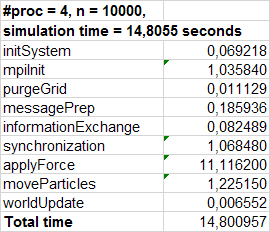
\includegraphics[width=\textwidth]{time.png}
    \caption{Time spent calculating.}
  \end{minipage}
\end{figure}

\section{Testing}
Code has been tested using a series of assertions, constantly confirming that the local grid for each process is correct. Likewise has the sdl visualization tool been used.

\chapter{Conclusion}


%-----------------------------------------------------------------
%						     APPENDIX
%-----------------------------------------------------------------
\newpage
\newgeometry{left=2.5cm,right=2.5cm}
\chapter{Appendix}
\section{Serial algorithm plotting data}

\begin{figure}[H]
  \centering
  \begin{minipage}[b]{0.9\textwidth}
    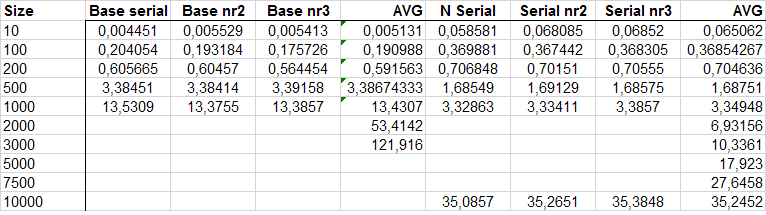
\includegraphics[width=\textwidth]{plotdata.png}
    \caption{Plotting data for the linear runtimes.}
  \end{minipage}
\end{figure}

\end{document}
